\documentclass[12pt, oneside, a4paper]{article}

\usepackage{authblk}
\usepackage{graphicx}
\usepackage{placeins}
\usepackage{amsmath}
\usepackage{needspace}
\usepackage{pdfpages}
\usepackage[colorlinks = true,
            linkcolor = blue,
            urlcolor  = blue,
            citecolor = blue,
            anchorcolor = blue]{hyperref}
%\usepackage[section]{placeins}

\parskip 3mm

\title{CRSU Startup}
\author{M.\ Rigan}
\affil{MPS, University of Sussex}
\date{\today}

\begin{document}
\maketitle
\begin{abstract}
		The details of the CRSU setup, preliminary checks, procedures to follow when starting up the control room and ideas are discussed in this document.
\end{abstract}
\clearpage
\tableofcontents
\clearpage

\section{Set Up}
\paragraph{•}
Machines abbreviations:
\begin{itemize}
	\item Operating machine (Mac) = \textbf{\texttt opersu}
	\item Monitoring machine 1 (CentOs) = \textbf{\texttt monsu1 }
	\item Monitoring machine 2 (CentOS) = \textbf{\texttt monsu2}
\end{itemize}
\begin{center}
%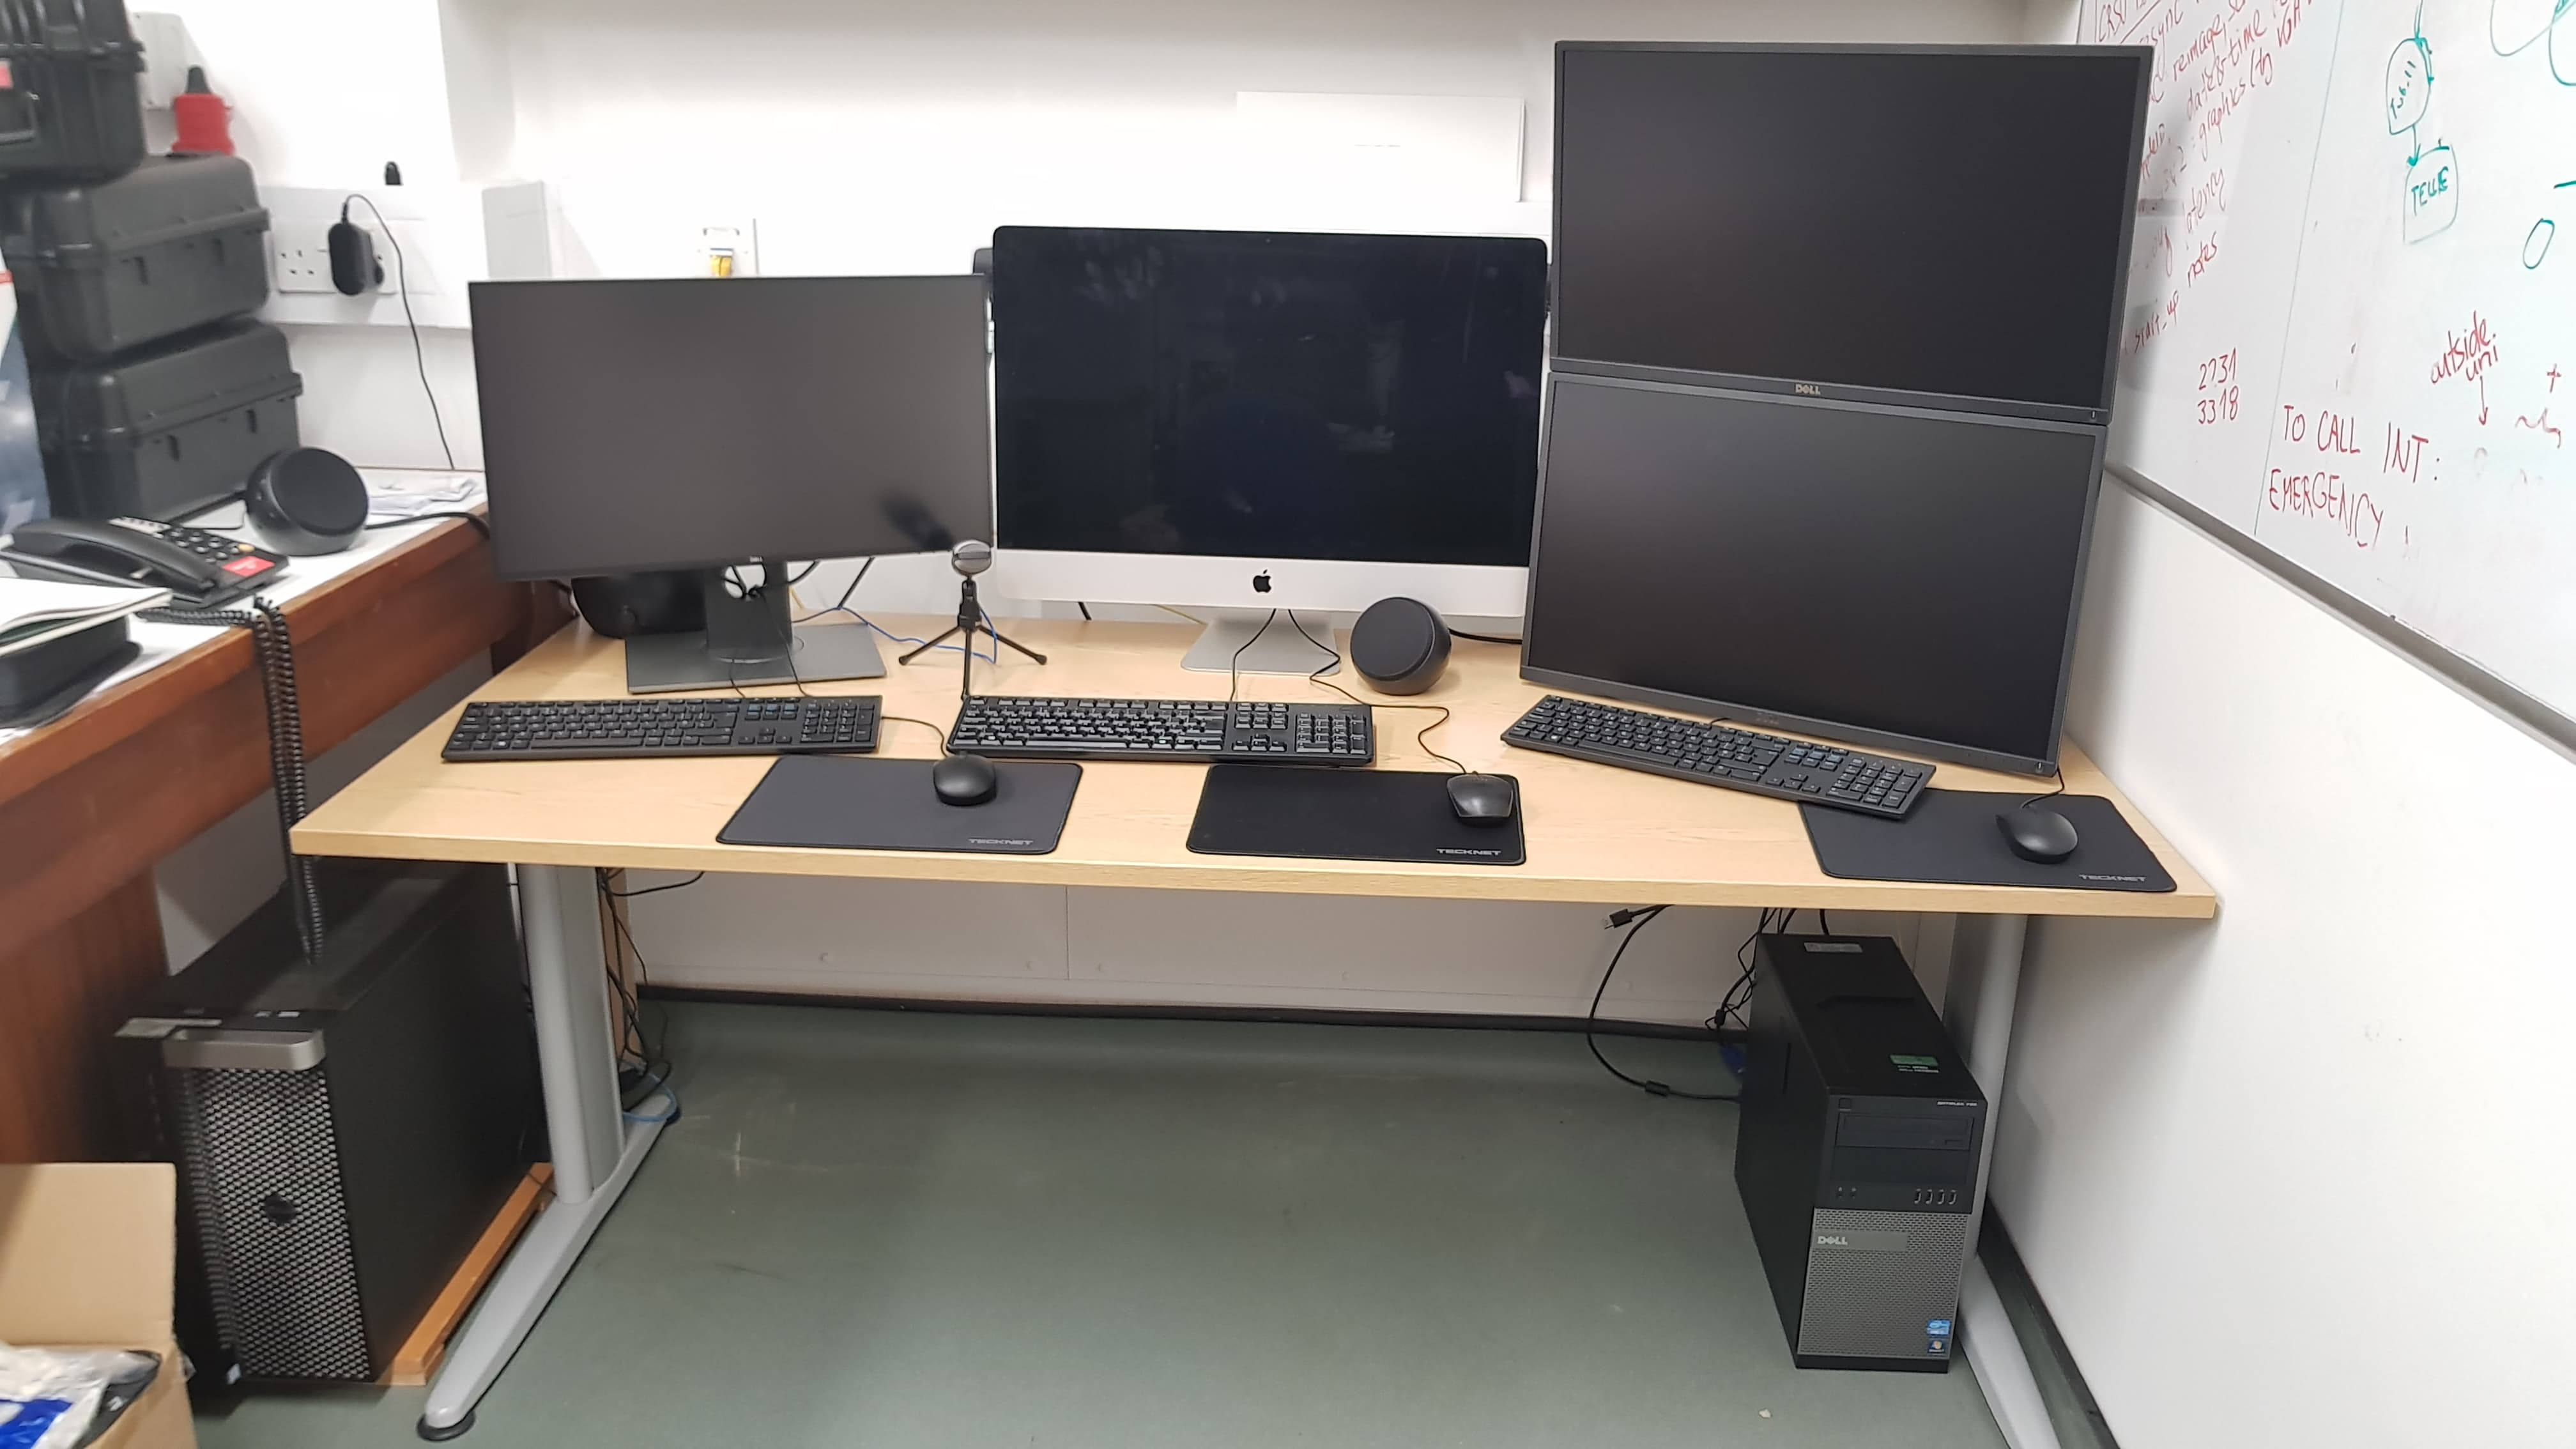
\includegraphics[width=1\textwidth]{figures/set_up.jpg} Figure 1: Current set-up of the remote control room
\end{center}
\paragraph{•}
{\texttt monsu1} is the machine on the bottom left, connected to the very left monitor and the left pair of peripherals. {\texttt opersu} is the central machine, with the machine in-built into the monitor, connected to the central pair of peripherals. {\texttt monsu2} is on the right, with the double display setup. The power buttons are on the top left of both {\texttt monsu} machines and on the bottom left (backside) of the operating machine. Note that {\texttt monsu1} can take longer time to boot-up due to the RAID system and dual boot setup. {\texttt monsu2 }sometimes warns about incorrect date settings on startup, just press F1 whenever you see the warning message. Additionally, there is Windows running on a Virtual Machine (VM) on {\texttt monsu1} and the process is described later in the document.
\paragraph{•}
All machines have the 2 usual accounts configured: the \textbf{\texttt snoperator} and the \textbf{\texttt snotdaq} account. For {\texttt monsu} machines, you need to enter the account name ({\texttt snoperator}) at login as well. Additionally, {\texttt root} acounts are available at the {\texttt monsu} machines. Contact the remote room experts:
\begin{itemize}
\item (\href{mailto:M.Nirkko@sussex.ac.uk}{M.Nirkko@sussex.ac.uk} + 44 7948 759 907
\item \href{mailto:M.Rigan@sussex.ac.uk}{M.Rigan@sussex.ac.uk})  +44 7467 380 455
\end{itemize}
if you require details or run into trouble.

\section{Preliminary}
This list notes the preliminary requirements needed to access the remote control room:
\begin{itemize}
	\item SALTO access card: this is a card that allows people to access the Pevensey II. It is needed to get to the building outside the normal working hours (especially important for graveyard shifts). Speak to Simon Peeters (\href{mailto:S.J.M.Peeters@sussex.ac.uk}{S.J.M.Peeters@sussex.ac.uk}).
	\item Access to the lab (SNO+ Laboratory - 4A23 room, 1st floor of the Pevensey II building) is code restricted.  Speak to Simon Peeters \newline (\href{mailto:S.J.M.Peeters@sussex.ac.uk}{S.J.M.Peeters@sussex.ac.uk}) to gain access.
	\item Your SNOLab account details to log in to the VPN software
	\item The snoperator password and the global collaboration log in details
\end{itemize}

\section{Long time (10 or more days)}
\paragraph{•}
Before a detector shift is taken at a remote shift station, the shifter must make sure that all the software is up to date on the operator and monitoring machines. This not a problem unique to remote stations - the software on site machines also has to be properly maintained - but there is a frequency of use difference. If a remote station has not been used for 10 or more days the following checklist should be completed. All checks and tests should be run the day before the scheduled shift.
\begin{itemize}
	\item \textbf{restart both machines}: this clears out the cache and temp files, frees up RAM, kills unwanted services and (possibly) allows updates to be installed
	\item log in as {\texttt snoperator}
	\item \textbf{restart the VPN}: this needs to be done on all machines. Find 'Cisco anyconnect VPN' (icon on the opersu apps dock (bottom of the screen) and monsu apps bar (top left)). Use your snolab account and log into SL-SNOPLUS for Opersu and Monsu and SL-GEN on Windows machine. Select 'Connect Anyway' if there is a pop-up.
	\item \textbf{check for updates}: \newline 
	MONSUs: System tab $\rightarrow$ Administration $\rightarrow$ Software Update \newline 
	MAC: the Apple symbol on apps bar $\rightarrow$ About This Mac $\rightarrow$ Software Update \newline 
	On {\texttt monsu} machines you can use aliases: \textit{update} and \textit{update-linux} \newline
      In the VM on {\texttt monsu1}, check if there are updates available using the window update icon in the bottom-right corners (there are none available if it is not there).
\end{itemize}

\section{Start Up}
\paragraph{•}
The usual procedure to start up all required software (the {\texttt monsu} machines have multiple virtual workspaces that you can navigate around using the CTRL + ALT + Arrows):
\begin{itemize}
	\item Start-up the physical machines
	\item Start-up Windows on the VirtualBox: On {\texttt monsu1} there is icon `Oracle VM VirtualBox' located on the top right of the desktop. Start the app, select Windows 7 Pro (either double click the item in the list on the left or click the 'Start' green arrow). Log in as snoperator. Connect to VPN using the `VPN Client' icon on the desktop. Connect to the \textbf{SL-GEN} group. (Connecting to the VPN on Virtual machine can result in disconnecting from another VPN on another machine - this is Cisco security to prevent from overloading. Be sure to reconnect and everything runs fine - it only disconnects once!). Start up the phone application by selecting the `IP Phone' icon on the desktop. Finally open the UPS platform using the bookmark in firefox web browser (the UPS platform only works on SL-GEN, therefore can only be opened on this VM)
	\item Connect to VPN software on all machines: Find 'Cisco anyconnect VPN' (icon on the opersu apps dock (bottom of the screen) and monsu apps bar (top left)). Use your snolab account and log into SL-SNOPLUS. Select `Connect Anyway' if there is a pop-up (again, check if you weren't disconnected randomly on other machines)
	\item For {\texttt monsu1}:
	\begin{itemize}
		\item Start up: Alarm GUI, FEC FIFO, MTC GUI, Supernova monitor, DAQ log and Builder log by clicking appropriate icons on the desktop (use multiple workspaces as appropriate). Sometimes a DB connection pop-up appears for the ALARM GUI (possibly other apps), use the collaboration log-in to connect. Supernova and Builder require the snoperator's password to connect.		
			\item Run Scope from the desktop (icon).
			\item This machine also runs Check Rates and Polling GUI when needed during the shift by selecting appropriate application on the desktop. List of all application is also available at Applications $\rightarrow$ Other from the taskbar.
		\item Make sure the virtual phone software is running on windows virtual machine as described above.
	\end{itemize}
	\item For {\texttt monsu2} (this machine is dedicated to run high-load streaming apps):
	\begin{itemize}
		\item run the local Dispatcher by clicking the icon on the desktop
		\item start 4 copies of XSNOED by clicking the icons on the desktop. There are specific icons to open Top or Bottom view xsnoed, each of which will open the application on the respective monitor. The suggested settings are: live, sum (-PED), 100 NHit and 500 NHit environments (again, use as many workspaces as you like)
		\item Open the Minard stream in browser (bookmarks provided)
\item be sure to have Slow control, Detector State, Detector State Check, Nearline monitor, PMT Calibration Summary, Grafana (data-flow) and the Weather forecast (blizzards) tabs open in a browser (bookmarks provided)

	\end{itemize}
\item For {\texttt opersu}:
	\begin{itemize}
		\item Connect to remote drive with orca files: 'Go' tab from the taskbar (top left) $\rightarrow$ Connect to Server. Select buffer1 from the Favorite Servers
		\item start TUBii audio by clicking the 'TUB\_audio.m3u' icon on the desktop. Be sure to disable video to decrease the load (Video $\rightarrow$ Video Track $\rightarrow$ Disable)
		\item When you are ready for the handover (after calling the previous shifter), right click the snot\_main.Orca file and select 'Open With' $\rightarrow$ Orca(default). This ensures the correct version of Orca is opened instead of using the icon in the App doc
		\item check correct version of Orca is running at \href{https://snopl.us/monitoring/orca-session-logs}{orca log}
	\end{itemize}
\item Be sure to have shift report page and Slack open at any of the machines (dedicated app installed at Mac)
\item To call international numbers (such as on-call expert), dial \newline 9-1470-00-\textit{number}
\end{itemize}

\section{In case of a fire alarm}

Make sure you have your mobile and a piece of paper with the expert's contact details.

\section{Ideas}
\begin{itemize}
	\item Global SALTO card for lab?
      \item Improve fire alarm procedure.
\end{itemize}

\end{document}